\documentclass[aspectratio=169]{beamer}

\usetheme{Madrid}
\usecolortheme{whale}

% Packages
\usepackage{graphicx}
\usepackage{tikz}
\usepackage{hyperref}
\usepackage{booktabs}
\usepackage{xcolor}
\usepackage{listings}

% Custom colors - Resilience Academy theme
\definecolor{raBlue}{RGB}{0, 166, 214}
\definecolor{raDarkBlue}{RGB}{0, 102, 153}
\definecolor{primaryblue}{RGB}{0, 102, 179}
\definecolor{secondarygreen}{RGB}{46, 139, 87}
\definecolor{accentorange}{RGB}{255, 140, 0}
\definecolor{codebg}{RGB}{245, 245, 245}

% Listings style for code
\lstset{
    backgroundcolor=\color{codebg},
    basicstyle=\ttfamily\tiny,
    breaklines=true,
    frame=single,
    language=Python,
    keywordstyle=\color{primaryblue},
    commentstyle=\color{secondarygreen},
    stringstyle=\color{accentorange}
}

% Title information
\title[Geospatial Visualization]{Geospatial Visualization Tools}
\subtitle{Tools, Examples \& Case Studies}
\author{Masoud Hamad}
\institute{School of Computing Communication and Media Studies\\Resilience Academy}
\date{2025}

\begin{document}

% Formal Title Slide
{
\setbeamertemplate{navigation symbols}{}
\begin{frame}[plain]
\begin{tikzpicture}[remember picture, overlay]
    % White background
    \fill[white] (current page.north west) rectangle (current page.south east);

    % Blue accent bar at top
    \fill[raBlue] (current page.north west) rectangle ([yshift=-1.5cm]current page.north east);

    % Blue accent bar at bottom
    \fill[raBlue] ([yshift=1.2cm]current page.south west) rectangle (current page.south east);

    % Resilience Academy text in top bar
    \node[anchor=west, white, font=\bfseries\large] at ([xshift=1cm, yshift=-0.75cm]current page.north west) {
        Resilience Academy
    };

    % Main Title
    \node[anchor=center, font=\fontsize{32}{36}\selectfont\bfseries, text width=14cm, align=center] at ([yshift=1.5cm]current page.center) {
        A Guide to \textcolor{raBlue}{Visualization}\\[0.3cm]
        Tools and Strategies
    };

    % Subtitle
    \node[anchor=center, font=\large, text=gray] at ([yshift=-0.5cm]current page.center) {
        Geospatial Data Visualization with Python
    };

    % Author
    \node[anchor=center, font=\Large\bfseries] at ([yshift=-2cm]current page.center) {
        Masoud Hamad
    };

    % Institution
    \node[anchor=center, font=\normalsize, text=gray, text width=12cm, align=center] at ([yshift=-3cm]current page.center) {
        School of Computing Communication and Media Studies\\[0.2cm]
        Resilience Academy
    };

    % Year in bottom bar
    \node[anchor=center, white, font=\bfseries] at ([yshift=0.6cm]current page.south) {
        2025
    };

    % Website
    \node[anchor=east, white, font=\small] at ([xshift=-1cm, yshift=0.6cm]current page.south east) {
        resilienceacademy.ac.tz
    };

\end{tikzpicture}
\end{frame}
}

% Outline
\begin{frame}{Outline}
    \tableofcontents
\end{frame}

%====================================
\section{Introduction to Geospatial Visualization}
%====================================

\begin{frame}{Why Geospatial Visualization?}
    \begin{columns}
        \column{0.5\textwidth}
        \textbf{Key Benefits:}
        \begin{itemize}
            \item Reveal spatial patterns and relationships
            \item Communicate complex data intuitively
            \item Support decision-making processes
            \item Enable exploratory data analysis
            \item Facilitate stakeholder engagement
        \end{itemize}

        \column{0.5\textwidth}
        \textbf{Applications:}
        \begin{itemize}
            \item Climate change monitoring
            \item Urban planning
            \item Disaster response
            \item Environmental conservation
            \item Public health epidemiology
            \item Transportation planning
        \end{itemize}
    \end{columns}
\end{frame}

\begin{frame}{Types of Geospatial Data}
    \begin{columns}
        \column{0.5\textwidth}
        \textbf{\color{primaryblue}Vector Data}
        \begin{itemize}
            \item \textbf{Points:} Cities, sensors, events
            \item \textbf{Lines:} Roads, rivers, pipelines
            \item \textbf{Polygons:} Countries, watersheds, parcels
        \end{itemize}
        \vspace{0.3cm}
        \textit{Formats:} GeoJSON, Shapefile, GeoPackage

        \column{0.5\textwidth}
        \textbf{\color{secondarygreen}Raster Data}
        \begin{itemize}
            \item Satellite imagery
            \item Digital elevation models (DEM)
            \item Land cover classifications
            \item Temperature/precipitation grids
        \end{itemize}
        \vspace{0.3cm}
        \textit{Formats:} GeoTIFF, NetCDF, COG
    \end{columns}
\end{frame}

%====================================
\section{Python Visualization Tools}
%====================================

\begin{frame}{Overview of Python Geospatial Stack}
    \centering
    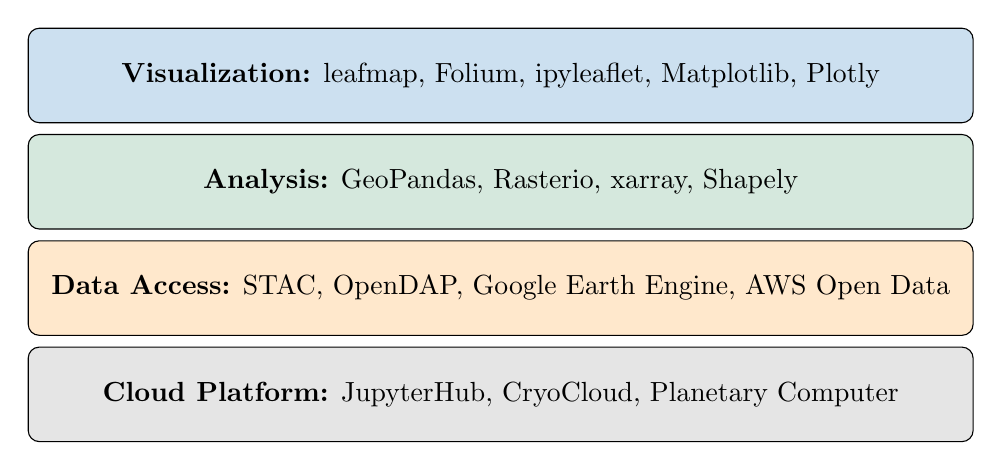
\begin{tikzpicture}[scale=0.9]
        % Visualization layer
        \node[draw, fill=primaryblue!20, minimum width=12cm, minimum height=1.2cm, rounded corners] at (0,3) {\textbf{Visualization:} leafmap, Folium, ipyleaflet, Matplotlib, Plotly};

        % Analysis layer
        \node[draw, fill=secondarygreen!20, minimum width=12cm, minimum height=1.2cm, rounded corners] at (0,1.5) {\textbf{Analysis:} GeoPandas, Rasterio, xarray, Shapely};

        % Data access layer
        \node[draw, fill=accentorange!20, minimum width=12cm, minimum height=1.2cm, rounded corners] at (0,0) {\textbf{Data Access:} STAC, OpenDAP, Google Earth Engine, AWS Open Data};

        % Cloud platform
        \node[draw, fill=gray!20, minimum width=12cm, minimum height=1.2cm, rounded corners] at (0,-1.5) {\textbf{Cloud Platform:} JupyterHub, CryoCloud, Planetary Computer};
    \end{tikzpicture}
\end{frame}

%------------------------------------
\subsection{leafmap}
%------------------------------------

\begin{frame}[fragile]{leafmap: Interactive Geospatial Mapping}
    \begin{columns}
        \column{0.55\textwidth}
        \textbf{Features:}
        \begin{itemize}
            \item Built on ipyleaflet and Folium
            \item Minimal coding required
            \item 400+ basemaps available
            \item Cloud Optimized GeoTIFF (COG) support
            \item Split-panel maps for comparison
            \item Integration with Google Earth Engine
            \item Time-series animation
        \end{itemize}

        \vspace{0.3cm}
        \textbf{Installation:}
\begin{lstlisting}
pip install leafmap
conda install -c conda-forge leafmap
\end{lstlisting}

        \column{0.45\textwidth}
        \textbf{Quick Example:}
\begin{lstlisting}
import leafmap

# Create interactive map
m = leafmap.Map(center=[40, -100],
                zoom=4)

# Add basemap
m.add_basemap("OpenTopoMap")

# Add GeoJSON layer
m.add_geojson("states.geojson",
    layer_name="US States")

# Display map
m
\end{lstlisting}
    \end{columns}
\end{frame}

\begin{frame}[fragile]{leafmap: Advanced Capabilities}
    \begin{columns}
        \column{0.5\textwidth}
        \textbf{Split Map Comparison:}
\begin{lstlisting}
import leafmap

m = leafmap.Map()
m.split_map(
    left_layer="TERRAIN",
    right_layer="SATELLITE"
)
m
\end{lstlisting}

        \vspace{0.3cm}
        \textbf{COG Visualization:}
\begin{lstlisting}
url = "https://example.com/cog.tif"
m.add_cog_layer(url,
    name="Cloud Optimized GeoTIFF")
\end{lstlisting}

        \column{0.5\textwidth}
        \textbf{Time-Series Animation:}
\begin{lstlisting}
images = [
    "2020_01.tif",
    "2020_06.tif",
    "2020_12.tif"
]
m.add_time_slider(
    images,
    labels=["Jan", "Jun", "Dec"],
    time_interval=1
)
\end{lstlisting}

        \vspace{0.3cm}
        \textbf{Use Cases:}
        \begin{itemize}
            \item Land cover change detection
            \item Flood extent mapping
            \item Urban growth analysis
        \end{itemize}
    \end{columns}
\end{frame}

%------------------------------------
\subsection{Folium}
%------------------------------------

\begin{frame}[fragile]{Folium: Leaflet.js for Python}
    \begin{columns}
        \column{0.5\textwidth}
        \textbf{Strengths:}
        \begin{itemize}
            \item Lightweight and fast
            \item Exports to standalone HTML
            \item Great for web deployment
            \item Choropleth maps
            \item Marker clusters
            \item Heatmaps
        \end{itemize}

        \column{0.5\textwidth}
        \textbf{Choropleth Example:}
\begin{lstlisting}
import folium
import pandas as pd

m = folium.Map(location=[40, -95],
               zoom_start=4)

folium.Choropleth(
    geo_data="us-states.json",
    data=df,
    columns=["State", "Population"],
    key_on="feature.id",
    fill_color="YlGn",
    legend_name="Population"
).add_to(m)

m.save("map.html")
\end{lstlisting}
    \end{columns}
\end{frame}

%------------------------------------
\subsection{GeoPandas \& Matplotlib}
%------------------------------------

\begin{frame}[fragile]{GeoPandas: Static Map Visualization}
    \begin{columns}
        \column{0.5\textwidth}
        \textbf{Features:}
        \begin{itemize}
            \item Extends Pandas for spatial data
            \item Publication-quality static maps
            \item Spatial operations (buffer, intersect)
            \item Multiple file format support
            \item Integration with Matplotlib
        \end{itemize}

        \column{0.5\textwidth}
        \textbf{Example:}
\begin{lstlisting}
import geopandas as gpd
import matplotlib.pyplot as plt

# Read shapefile
gdf = gpd.read_file("countries.shp")

# Plot with styling
fig, ax = plt.subplots(figsize=(12, 8))
gdf.plot(
    column="population",
    cmap="viridis",
    legend=True,
    ax=ax
)
ax.set_title("World Population")
plt.savefig("map.png", dpi=300)
\end{lstlisting}
    \end{columns}
\end{frame}

%------------------------------------
\subsection{Plotly}
%------------------------------------

\begin{frame}[fragile]{Plotly: Interactive Statistical Maps}
    \begin{columns}
        \column{0.5\textwidth}
        \textbf{Capabilities:}
        \begin{itemize}
            \item Interactive zoom and pan
            \item Hover tooltips
            \item Scatter geo plots
            \item Choropleth maps
            \item 3D globe visualization
            \item Dash integration for apps
        \end{itemize}

        \column{0.5\textwidth}
        \textbf{Scatter Geo Example:}
\begin{lstlisting}
import plotly.express as px

df = px.data.gapminder()

fig = px.scatter_geo(
    df,
    locations="iso_alpha",
    size="pop",
    color="continent",
    hover_name="country",
    animation_frame="year",
    projection="natural earth"
)
fig.show()
\end{lstlisting}
    \end{columns}
\end{frame}

%====================================
\section{Desktop \& Web-Based Tools}
%====================================

\begin{frame}[fragile]{QGIS: Open Source Desktop GIS}
    \begin{columns}
        \column{0.5\textwidth}
        \textbf{Key Features:}
        \begin{itemize}
            \item Free and open source
            \item 500+ plugins available
            \item Print composer for cartography
            \item 3D visualization
            \item Raster and vector analysis
            \item Python scripting (PyQGIS)
            \item Database connectivity
        \end{itemize}

        \vspace{0.3cm}
        \textbf{Best For:}
        \begin{itemize}
            \item Complex cartographic outputs
            \item Data editing and digitizing
            \item Geoprocessing workflows
        \end{itemize}

        \column{0.5\textwidth}
        \textbf{PyQGIS Example:}
\begin{lstlisting}
from qgis.core import *
from qgis.utils import iface

# Load vector layer
layer = QgsVectorLayer(
    "path/to/file.shp",
    "Layer Name",
    "ogr"
)

# Add to map canvas
QgsProject.instance().addMapLayer(layer)

# Apply graduated symbology
renderer = QgsGraduatedSymbolRenderer()
renderer.setClassAttribute("population")
layer.setRenderer(renderer)
\end{lstlisting}
    \end{columns}
\end{frame}

\begin{frame}[fragile]{Kepler.gl: Large-Scale Geospatial Visualization}
    \begin{columns}
        \column{0.5\textwidth}
        \textbf{Features:}
        \begin{itemize}
            \item GPU-powered rendering
            \item Handles millions of points
            \item 3D visualizations
            \item Time-series playback
            \item Arc, hexbin, heatmap layers
            \item Export to HTML/JSON
            \item Jupyter integration
        \end{itemize}

        \vspace{0.2cm}
        \textbf{Best For:}
        \begin{itemize}
            \item Big data visualization
            \item Movement/trajectory data
            \item Urban analytics
        \end{itemize}

        \column{0.5\textwidth}
        \textbf{Python Example:}
\begin{lstlisting}
from keplergl import KeplerGl
import pandas as pd

# Load data
df = pd.read_csv("taxi_trips.csv")

# Create map
map_1 = KeplerGl(height=600)

# Add data
map_1.add_data(data=df,
               name="NYC Taxi Trips")

# Display
map_1
\end{lstlisting}

        \vspace{0.2cm}
        \url{https://kepler.gl}
    \end{columns}
\end{frame}

\begin{frame}[fragile]{Google Earth Engine: Planetary-Scale Analysis}
    \begin{columns}
        \column{0.5\textwidth}
        \textbf{Capabilities:}
        \begin{itemize}
            \item Petabytes of satellite imagery
            \item Cloud-based processing
            \item Time-series analysis
            \item Machine learning integration
            \item JavaScript and Python APIs
            \item Free for research/education
        \end{itemize}

        \vspace{0.2cm}
        \textbf{Available Datasets:}
        \begin{itemize}
            \item Landsat (1972--present)
            \item Sentinel-1/2
            \item MODIS products
            \item Climate data (ERA5, CHIRPS)
        \end{itemize}

        \column{0.5\textwidth}
        \textbf{Python API Example:}
\begin{lstlisting}
import ee
import geemap

ee.Initialize()

# Load Sentinel-2 imagery
s2 = ee.ImageCollection("COPERNICUS/S2") \
    .filterDate("2023-01-01", "2023-12-31") \
    .filterBounds(geometry) \
    .filter(ee.Filter.lt(
        "CLOUDY_PIXEL_PERCENTAGE", 20)) \
    .median()

# Visualize with geemap
Map = geemap.Map()
Map.addLayer(s2,
    {"bands": ["B4", "B3", "B2"],
     "max": 3000}, "RGB")
Map
\end{lstlisting}
    \end{columns}
\end{frame}

%====================================
\section{Case Studies}
%====================================

\begin{frame}{Case Study 1: Urban Heat Island Analysis}
    \begin{columns}
        \column{0.55\textwidth}
        \textbf{Objective:}
        Map urban heat islands in Phoenix, AZ using Landsat thermal data

        \vspace{0.3cm}
        \textbf{Tools Used:}
        \begin{itemize}
            \item Google Earth Engine (data access)
            \item leafmap (visualization)
            \item GeoPandas (vector overlays)
        \end{itemize}

        \vspace{0.3cm}
        \textbf{Workflow:}
        \begin{enumerate}
            \item Acquire Landsat 8/9 thermal bands
            \item Calculate Land Surface Temperature
            \item Classify heat intensity zones
            \item Overlay with land use data
            \item Create split-map visualization
        \end{enumerate}

        \column{0.45\textwidth}
        \textbf{Key Findings:}
        \begin{itemize}
            \item Downtown 5--8 degrees C warmer than suburbs
            \item Parks show 3--4 degrees C cooling effect
            \item Correlation with impervious surfaces
        \end{itemize}

        \vspace{0.3cm}
        \textbf{Impact:}
        \begin{itemize}
            \item Informed city tree planting program
            \item Updated building codes for cool roofs
            \item Public health heat warnings
        \end{itemize}
    \end{columns}
\end{frame}

\begin{frame}{Case Study 2: Flood Risk Mapping}
    \begin{columns}
        \column{0.5\textwidth}
        \textbf{Objective:}
        Create interactive flood risk maps for Houston, TX

        \vspace{0.3cm}
        \textbf{Tools Used:}
        \begin{itemize}
            \item QGIS (hydrological analysis)
            \item Folium (web map creation)
            \item Plotly (statistical charts)
        \end{itemize}

        \vspace{0.3cm}
        \textbf{Data Sources:}
        \begin{itemize}
            \item USGS National Elevation Dataset
            \item FEMA flood zones
            \item Census block population data
            \item Historical flood events
        \end{itemize}

        \column{0.5\textwidth}
        \textbf{Methodology:}
        \begin{enumerate}
            \item Generate flow accumulation raster
            \item Delineate flood-prone areas
            \item Calculate population exposure
            \item Build interactive dashboard
        \end{enumerate}

        \vspace{0.3cm}
        \textbf{Deliverables:}
        \begin{itemize}
            \item Web-based risk explorer
            \item Downloadable reports by ZIP code
            \item API for emergency services
            \item Mobile-friendly interface
        \end{itemize}
    \end{columns}
\end{frame}

\begin{frame}[fragile]{Case Study 3: Deforestation Monitoring}
    \begin{columns}
        \column{0.5\textwidth}
        \textbf{Objective:}
        Track deforestation in the Amazon using time-series satellite data

        \vspace{0.3cm}
        \textbf{Tools Used:}
        \begin{itemize}
            \item Google Earth Engine (processing)
            \item geemap (visualization)
            \item Kepler.gl (change animation)
        \end{itemize}

        \vspace{0.3cm}
        \textbf{Analysis Pipeline:}
        \begin{enumerate}
            \item Collect Sentinel-2 monthly composites
            \item Calculate NDVI time series
            \item Detect forest loss events
            \item Generate change statistics
            \item Create animated visualization
        \end{enumerate}

        \column{0.5\textwidth}
        \textbf{Code Snippet:}
\begin{lstlisting}
# NDVI calculation
def addNDVI(image):
    ndvi = image.normalizedDifference(
        ['B8', 'B4']).rename('NDVI')
    return image.addBands(ndvi)

# Apply to collection
ndvi_collection = s2.map(addNDVI)

# Detect change
change = ndvi_2023.subtract(ndvi_2020)
deforestation = change.lt(-0.3)
\end{lstlisting}

        \vspace{0.2cm}
        \textbf{Results:}
        \begin{itemize}
            \item 12,000 sq km loss detected (2020--2023)
            \item Near real-time alert system
        \end{itemize}
    \end{columns}
\end{frame}

\begin{frame}[fragile]{Case Study 4: COVID-19 Spread Visualization}
    \begin{columns}
        \column{0.5\textwidth}
        \textbf{Objective:}
        Visualize pandemic spread patterns and healthcare access

        \vspace{0.3cm}
        \textbf{Tools Used:}
        \begin{itemize}
            \item Plotly (animated choropleth)
            \item Folium (hospital locations)
            \item GeoPandas (spatial analysis)
        \end{itemize}

        \vspace{0.3cm}
        \textbf{Visualizations Created:}
        \begin{itemize}
            \item Animated case count maps
            \item Hospital catchment areas
            \item Vaccination coverage maps
            \item Mobility change heatmaps
        \end{itemize}

        \column{0.5\textwidth}
        \textbf{Animated Map Code:}
\begin{lstlisting}
fig = px.choropleth(
    df,
    locations="state",
    locationmode="USA-states",
    color="cases_per_100k",
    animation_frame="date",
    color_continuous_scale="Reds",
    range_color=[0, 500],
    scope="usa",
    title="COVID-19 Cases per 100K"
)
fig.update_layout(
    geo=dict(showlakes=False)
)
\end{lstlisting}

        \vspace{0.2cm}
        \textbf{Impact:} Informed resource allocation
    \end{columns}
\end{frame}

%====================================
\section{Tool Comparison}
%====================================

\begin{frame}{Tool Selection Guide}
    \centering
    \footnotesize
    \begin{tabular}{l|c|c|c|c|c}
        \toprule
        \textbf{Feature} & \textbf{leafmap} & \textbf{Folium} & \textbf{Plotly} & \textbf{Kepler.gl} & \textbf{QGIS} \\
        \midrule
        Interactive & Yes & Yes & Yes & Yes & Limited \\
        Big Data & Good & Limited & Good & Excellent & Good \\
        3D Support & Basic & No & Yes & Yes & Yes \\
        Code-free & No & No & No & Yes & Yes \\
        Web Export & Yes & Yes & Yes & Yes & Plugin \\
        COG Support & Yes & No & No & No & Yes \\
        GEE Integration & Yes & No & No & No & Plugin \\
        Learning Curve & Low & Low & Medium & Low & High \\
        \bottomrule
    \end{tabular}

    \vspace{0.5cm}
    \textbf{Recommendations:}
    \begin{itemize}
        \item \textbf{Quick exploration:} leafmap or Kepler.gl
        \item \textbf{Web deployment:} Folium or Plotly
        \item \textbf{Big data:} Kepler.gl
        \item \textbf{Print cartography:} QGIS
        \item \textbf{Cloud data:} leafmap + Google Earth Engine
    \end{itemize}
\end{frame}

%====================================
\section{Best Practices}
%====================================

\begin{frame}{Visualization Best Practices}
    \begin{columns}
        \column{0.5\textwidth}
        \textbf{\color{primaryblue}Design Principles:}
        \begin{itemize}
            \item Choose appropriate projections
            \item Use color-blind friendly palettes
            \item Include scale bars and north arrows
            \item Provide clear legends
            \item Minimize visual clutter
            \item Consider your audience
        \end{itemize}

        \vspace{0.3cm}
        \textbf{\color{secondarygreen}Color Schemes:}
        \begin{itemize}
            \item Sequential: Single variable intensity
            \item Diverging: Values above/below center
            \item Qualitative: Categorical data
        \end{itemize}

        \column{0.5\textwidth}
        \textbf{\color{accentorange}Performance Tips:}
        \begin{itemize}
            \item Simplify geometries for web
            \item Use vector tiles for large datasets
            \item Implement level-of-detail rendering
            \item Cache frequently accessed data
            \item Use Cloud Optimized formats (COG, COPC)
        \end{itemize}

        \vspace{0.3cm}
        \textbf{Accessibility:}
        \begin{itemize}
            \item Alt text for static maps
            \item Keyboard navigation
            \item High contrast options
            \item Screen reader compatibility
        \end{itemize}
    \end{columns}
\end{frame}

%====================================
\section{Resources}
%====================================

\begin{frame}{Learning Resources}
    \begin{columns}
        \column{0.5\textwidth}
        \textbf{Documentation:}
        \begin{itemize}
            \item leafmap.org
            \item python-visualization.github.io/folium
            \item plotly.com/python
            \item geopandas.org
            \item docs.kepler.gl
        \end{itemize}

        \vspace{0.3cm}
        \textbf{Tutorials:}
        \begin{itemize}
            \item Geospatial Python Course (leafmap)
            \item Google Earth Engine Guides
            \item Automating GIS Processes (U Helsinki)
        \end{itemize}

        \column{0.5\textwidth}
        \textbf{Data Sources:}
        \begin{itemize}
            \item \textbf{Resilience Academy CRD}\\
                  {\small crd.resilienceacademy.ac.tz}
            \item NASA Earthdata
            \item Copernicus Open Access Hub
            \item USGS Earth Explorer
            \item Microsoft Planetary Computer
        \end{itemize}

        \vspace{0.3cm}
        \textbf{Community:}
        \begin{itemize}
            \item GIS Stack Exchange
            \item r/gis (Reddit)
            \item OpenGeo Slack
            \item Pangeo community
        \end{itemize}
    \end{columns}
\end{frame}

\begin{frame}{Summary}
    \begin{columns}
        \column{0.6\textwidth}
        \textbf{Key Takeaways:}
        \begin{enumerate}
            \item Multiple tools exist for different use cases
            \item Python ecosystem is mature and well-integrated
            \item Cloud platforms enable large-scale analysis
            \item Interactive visualizations improve communication
            \item Open source tools match commercial capabilities
        \end{enumerate}

        \vspace{0.3cm}
        \textbf{Getting Started:}
        \begin{enumerate}
            \item Install leafmap for quick exploration
            \item Learn GeoPandas for data manipulation
            \item Explore Google Earth Engine for satellite data
            \item Use Folium/Plotly for web deployment
        \end{enumerate}

        \column{0.4\textwidth}
        \centering
        \vspace{1cm}
        \textbf{\Large Questions?}

        \vspace{1cm}
        \textbf{Workshop Website:}\\
        \small Visualization Challenge 2025

        \vspace{0.5cm}
        GitHub: massoudhamad/visualization
    \end{columns}
\end{frame}

\end{document}
